

\begin{frame}[fragile,label=1BmispredEx]{exercise (1)}
\begin{itemize}
\item use 1-bit predictor on this loop
\item what is the conditional jump misprediction rate?
\end{itemize}
\begin{lstlisting}[language=C,style=small]
int i = 0;
while (true) {
  if (i % 3 == 0) goto next; 
  ...
next:
  if (i % 10 > 2) goto next2; 
  ...
next2:
  i += 1;
}
\end{lstlisting}
\end{frame}

\ifdefined\exCode\else\newsavebox\exCode\fi
\begin{lrbox}{\exCode}
\begin{lstlisting}[language=C,style=smaller]
int i = 0;
while (true) {
  if (i % 3 == 0) goto next;
  ...
next:
  i += 1;
  if (i == 50) break;
}
\end{lstlisting}
\end{lrbox}

\begin{frame}<0>[fragile,label=1BmispredExSoln]{exercise soln (1)}
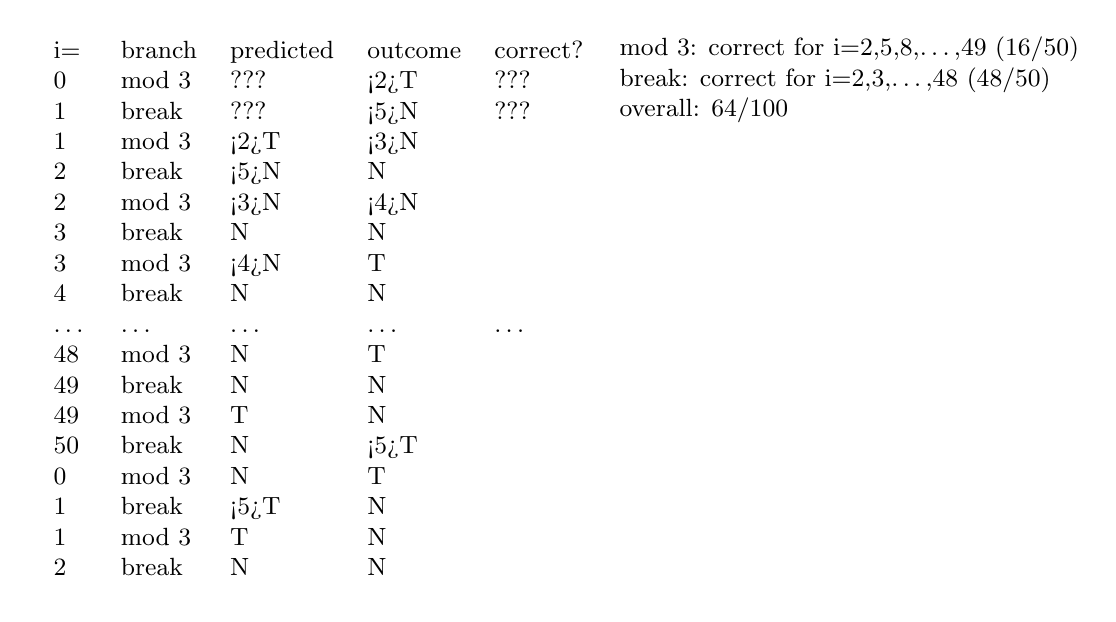
\begin{tikzpicture}
\node[font=\small] (table) {
\begin{tabular}{lllll}
i= & branch & predicted & outcome & correct? \\
0 & mod 3 & ??? & \myemph<2>{T} & ???\\
1 & break & ??? & \myemph<5>{N} & ???\\
1 & mod 3 & \myemph<2>{T} & \myemph<3>{N} & \\
2 & break & \myemph<5>{N} & N & \checkmark \\
2 & mod 3 & \myemph<3>{N} & \myemph<4>{N} & \checkmark \\
3 & break & N & N & \checkmark \\
3 & mod 3 & \myemph<4>{N} & T &\\
4 & break & N & N & \checkmark \\
\ldots & \ldots & \ldots & \ldots  & \ldots \\
48 & mod 3 & N & T & \\
49 & break & N & N & \checkmark \\
49 & mod 3 & T & N &\\
50 & break & N & \myemph<5>{T} & \\
0 & mod 3 & N & T &\\
1 & break & \myemph<5>{T} & N &\\
1 & mod 3 & T & N & \\
2 & break & N & N & \checkmark \\
\end{tabular}
};
\node[anchor=north west,align=left,font=\small](conclude) at (table.north east) {
mod 3: correct for i=2,5,8,\ldots,49 (16/50) \\
break: correct for i=2,3,\ldots,48 (48/50) \\
overall: 64/100
};
\node[anchor=north west] at (conclude.south west) {
    \usebox{\exCode}
};
\end{tikzpicture}
\end{frame}

